\lesson{Representing Enthalpy Changes}
The equations used to represent enthapy changes are called \textbf{thermochemical equations}.
For instance, the decomposition of water
\[
    \ch{H2O_{(\ell)}}\to \ch{H2_{(g)}}+\frac{1}{2}\ch{O2_{(g)}}\quad\Delta H_\text{decomp}=+285.8\,\si{kJ.mol^{-1}}\,\ch{H2O}
\]
The law of conservation of energy implies that the reverse is also true, only with a opposite
enthapy energy change
\[
    \ch{H2_{(g)}}+\frac{1}{2}\ch{O2_{(g)}}\to \ch{H2O_{(\ell)}}\quad\Delta H_\text{comb}=-285.8\,\si{kJ.mol^{-1}}\,\ch{H2}
\]
Since the former is endothermic, the enthalpy change is positive, while the latter is exothermic,
so the enthalpy change is negative. There are four main ways to represent energy changes
\begin{enum}
    \item Thermochemical equations with energy terms
    \item Thermochemical equations with $\Delta H$ values
    \item Molar enthalpies of reactions
    \item Potential energy diagrams
\end{enum}

\subsection{Method 1: Thermochemical Equations with Energy Terms}
In this method, we add the energy as a reactant/product into the BCE. For instance,
in the electrolysis of water 
\[
    \ch{H2O_{(\ell)}}+285.5\,\si{kJ}\to \ch{H2_{(g)}}+\frac{1}{2}\ch{O2_{(g)}}
\]
In this case, the energy is a reactant, which means the reaction is endothermic. In the case where
the reaction is exothermic, for instance in the synthesis of magnesium oxide
\[
    \ch{Mg_{(s)}}+\frac{1}{2}\ch{O2_{(g)}}\to \ch{MgO_{(s)}}+601.6\,\si{kJ}
\]
In this case, the energy is a product, which means the reaction is exothermic.

\begin{sample}{Write a thermochemical equation to represent the exothermic reaction that occurs
    when two moles of butane burn in excess oxygen gas. The molar enthalpy of combustion butane
    is -2871 \si{kJ.mol^{-1}}}
    The BCE is
    \[
        \ch{2C4H10_{(g)}}+13\ch{O2_{(g)}}\to 8 \ch{CO2_{(g)}}+10 \ch{H2O_{(g)}}
    \]
    Using mole ratios
    \begin{align*}
        \Delta H_\text{comb}&=2\,\si{mol}\times-2871\,\si{kJ.mol^{-1}}]\\
                            &=-5742\,\si{kJ}
    \end{align*}
    Therefore, since this is an exothermic reaction, the thermochemical equation is
    \[
        \ch{2C4H10_{(g)}}+13\ch{O2_{(g)}}\to 8 \ch{CO2_{(g)}}+10 \ch{H2O_{(g)}}+5742\,\si{kJ}
    \]
\end{sample}

\begin{sample}{Write a thermochemical equation to represent the dissolving of one mole of silver
    nitrate in water. The molar enthalpy of solution is +22.6 \si{kJ.mol^{-1}}}
    This is an endothermic reaction
    \[
        \ch{AgNO3_{(s)}}+22.6\,\si{kJ.mol^{-1}}\to \ch{Ag^+_{(aq)}}+\ch{NO3^-_{(aq)}}
    \]
\end{sample}

\subsection{Method 2: Thermochemical Equations with $\Delta H$ Values}
This method involves writing a BCE and then the $\Delta H_x$ value beside it. 

\begin{sample}{Sulfur dioxide and oxygen react to form sulfur trioxide. The molar enthalpy for the
        combustion of sulfur dioxide, $\Delta H_\text{comb}$, in this reaction is $-98.9\,\si{kJ.mol^{-1}}$.
        What is the enthalpy change for this reaction?
    }
    The BCE is
    \[
        2\ch{SO2}+\ch{O2}\to 2\ch{SO3}
    \]
    Therefore, with mole ratios
    \begin{align*}
        \Delta H&=2\,\si{mol}\times-98.9\,\si{kJ.mol^{-1}}\\
                &=-197.8\,\si{kJ}
    \end{align*}
    Therefore, the thermochemical equation is
    \[
        2\ch{SO2}+\ch{O2}\to 2\ch{SO3}\quad\Delta H=197.8\,\si{kJ}
    \]
\end{sample}

\begin{sample}{Write a thermochemical reaction, including a $\Delta H$ value, to represent the
    exothermic reaction between xenon gas and fluorine gas to produce solid xenon tetrafluoride,
    given that the reaction produces 251 kJ per mole of Xe reacted.}
    \[
        \ch{Xe_{(g)}}+2\ch{F2_{(g)}}\to \ch{XeF4_{(s)}}\quad\Delta H=-251\,\si{kJ}
    \]
\end{sample}

\subsection{Method 3: Molar Enthalpies of Reaction}
The \textbf{standard molar enthalpy of reaction} is molar enthalpy that is determined when the
initial and final conditiions of the chemical systems are at SATP. The symbol $\Delta H^\circ_x$
distinguishes standard molar enthalpies from molar enthalpies, $\Delta H_x$. The table below
shows some molar enthalpies of a reaction
\begin{figure}[ht!]
    \centering
    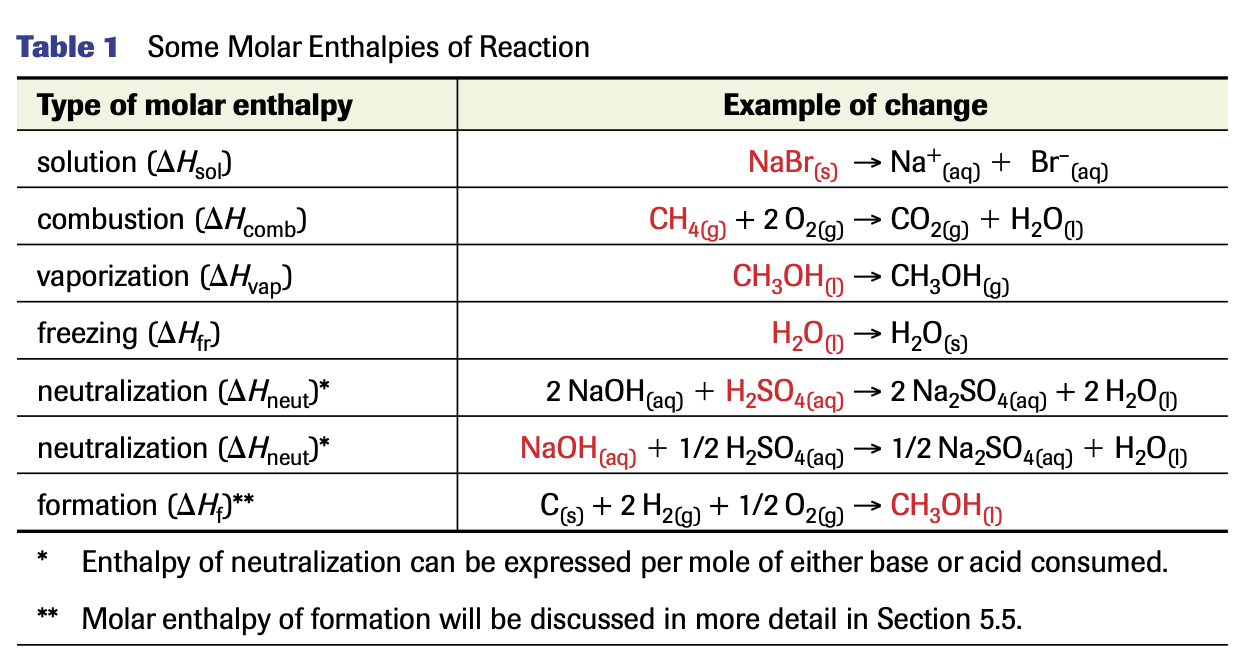
\includegraphics[width=0.8\textwidth]{../figures/molar-enthalpies-of-reaction.png}
\end{figure}
For an exothermic reaction, the standard molar enthalpy is measured by taking into account all
the energy required to change the reaction system from SATP; in order to intitiate the reaction,
and all the energy released following the reaction, as the products are cooled to SATP. For
instance, the synthesis to form methanol
\[
    \ch{CO_{(g)}}+2 \ch{H2_{(g)}}\to \ch{CH3OH_{(\ell)}}\quad\Delta H^\circ_r=-128.6\,\si{kJ.mol^{-1}}
\]

\subsection{Method 4: Potential Energy Diagrams}
This is a visual method of communicating energy transferred by using a \textbf{potential energy
diagram}. In this theoretical description, the energy transferred during a change is represented
as changes in the chemical potential energy of the particles as bonds are broken or formed.\\

\begin{figure}[ht!]
    \centering
    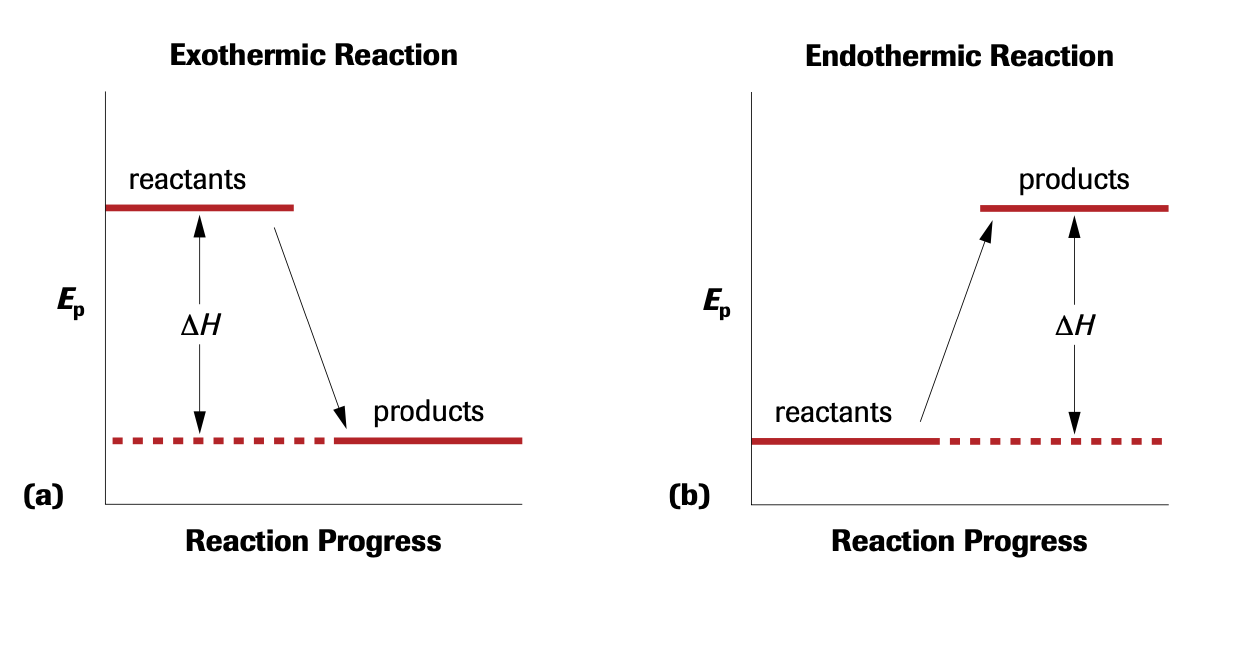
\includegraphics[width=0.8 \textwidth]{../figures/potential-energy-diagrams-1.png}
    \caption{During an exothermic reaction, the products have less potential energy than the
        reactants. During an endothermic reaction, the products have more potential energy than
        the reactants.}
\end{figure}

\begin{figure}[ht!]
    \centering
    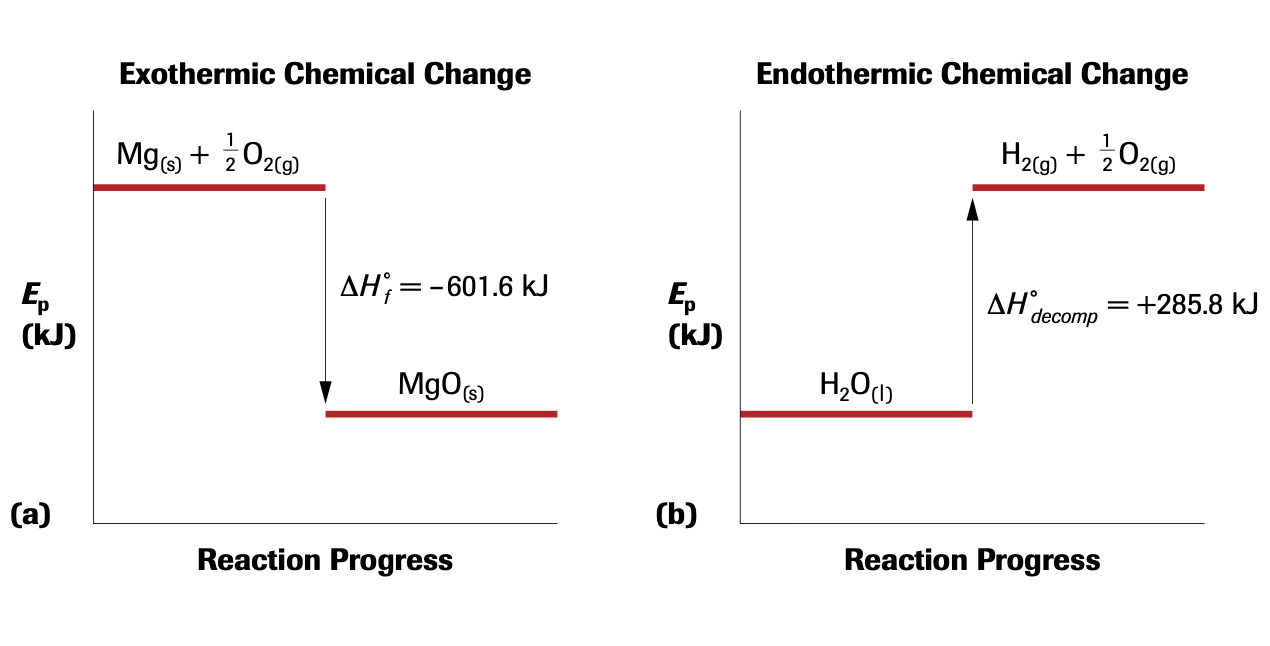
\includegraphics[width=0.8 \textwidth]{../figures/potential-energy-diagrams-2.png}
    \caption{In (a), it is a exothermic reaction in which one mole of magnesium oxide is formed. 
        In (b), it is an endothermic reaction in which water decomposes to hydrogen and oxygen.}
\end{figure}


